%%%%%%%%%%%%%%%%%%%%%%%%%%%%%%%%%%%%%%%%%%%%%%%%%%%%%%%%%%%%%%%%%%
%%%%%%%% ICML 2017 EXAMPLE LATEX SUBMISSION FILE %%%%%%%%%%%%%%%%%
%%%%%%%%%%%%%%%%%%%%%%%%%%%%%%%%%%%%%%%%%%%%%%%%%%%%%%%%%%%%%%%%%%

% Use the following line _only_ if you're still using LaTeX 2.09.
%\documentstyle[icml2017,epsf,natbib]{article}
% If you rely on Latex2e packages, like most moden people use this:
\documentclass{article}

% use Times
\usepackage{times}
% For figures
\usepackage{graphicx} % more modern
%\usepackage{epsfig} % less modern
\usepackage{subfigure} 

% For citations
\usepackage{natbib}

% For algorithms
\usepackage{algorithm}
\usepackage{algorithmic}

% As of 2011, we use the hyperref package to produce hyperlinks in the
% resulting PDF.  If this breaks your system, please commend out the
% following usepackage line and replace \usepackage{icml2017} with
% \usepackage[nohyperref]{icml2017} above.
\usepackage{hyperref}

% Packages hyperref and algorithmic misbehave sometimes.  We can fix
% this with the following command.
\newcommand{\theHalgorithm}{\arabic{algorithm}}

% Employ the following version of the ``usepackage'' statement for
% submitting the draft version of the paper for review.  This will set
% the note in the first column to ``Under review.  Do not distribute.''
\usepackage[accepted]{icml2017} 

% Employ this version of the ``usepackage'' statement after the paper has
% been accepted, when creating the final version.  This will set the
% note in the first column to ``Proceedings of the...''
%\usepackage[accepted]{icml2017}


% The \icmltitle you define below is probably too long as a header.
% Therefore, a short form for the running title is supplied here:
\icmltitlerunning{Effect of Signal Sparsity, Signal Density and Noise Level on Rotational Equivariant Features for Image Classification}

\begin{document} 

\twocolumn[
\icmltitle{Effect of Signal Sparsity, Signal Density and Noise Level on Rotational Equivariant Features for Image Classification}

% It is OKAY to include author information, even for blind
% submissions: the style file will automatically remove it for you
% unless you've provided the [accepted] option to the icml2017
% package.

% list of affiliations. the first argument should be a (short)
% identifier you will use later to specify author affiliations
% Academic affiliations should list Department, University, City, Region, Country
% Industry affiliations should list Company, City, Region, Country

% you can specify symbols, otherwise they are numbered in order
% ideally, you should not use this facility. affiliations will be numbered
% in order of appearance and this is the preferred way.



\icmlsetsymbol{equal}{*}

\begin{icmlauthorlist}
\icmlauthor{Aliraza Punjani}{}
\icmlauthor{Apoorv Kulshreshtha}{}
\icmlauthor{Jamshed Shapoorjee}{}
\icmlauthor{Plaban Mohanty}{}
\end{icmlauthorlist}
\begin{center}
\{ amp2280, ak3963, js4962, pm2878 \}@columbia.edu
\end{center}
%\icmlaffiliation{to}{University of Torontoland, Torontoland, Canada}
%\icmlaffiliation{goo}{Googol ShallowMind, New London, Michigan, USA}
%\icmlaffiliation{ed}{University of Edenborrow, Edenborrow, United Kingdom}

\icmlcorrespondingauthor{Aliraza}{amp2280@columbia.edu}
\icmlcorrespondingauthor{Apoorv}{ak3963@columbia.edu}
\icmlcorrespondingauthor{Jamshed}{js4962@columbia.edu}
\icmlcorrespondingauthor{Plaban}{pm2878@columbia.edu}

% You may provide any keywords that you 
% find helpful for describing your paper; these are used to populate 
% the "keywords" metadata in the PDF but will not be shown in the document
\icmlkeywords{boring formatting information, machine learning, ICML}

\vskip 0.2in
]

% this must go after the closing bracket ] following \twocolumn[ ...

% This command actually creates the footnote in the first column
% listing the affiliations and the copyright notice.
% The command takes one argument, which is text to display at the start of the footnote.
% The \icmlEqualContribution command is standard text for equal contribution.
% Remove it (just {}) if you do not need this facility.

%\printAffiliationsAndNotice{}  % leave blank if no need to mention equal contribution
%\printAffiliationsAndNotice{\icmlEqualContribution} % otherwise use the standard text.
%\footnotetext{hi}





\begin{abstract} 
Current convolution methods for feature learning are already translation equivariant i.e. translation in input image produces a proportionate translation in feature maps. However, this is not true for rotational equivariance. A lot of recent research has been focussed on ensuring rotational equivariance for the same. Our research focusses on characterizing effect of different input image parameters, like sparsity, density and noise, on effectiveness of the learnt rotational equivariant features proposed in the recent work of Harmonic Convolutions. Feature maps learnt using Harmonic Convolutions exhibit equivariance to patch-wise translation and 360 degree rotation. These variant of normal convolutions use parameter-efficient and low computational complexity representation, thereby encoding complicated rotational equivariance within the network. In this paper, we show the effectiveness of rotational equivariance features for image classification as the sparsity, density and noise levels of the input image vary.

\end{abstract} 

\section{Introduction}
Traditional convolutional networks are one of the popular methods for Image Classification. Due to various advancements over the years and the availability of more computational power convolutional neural networks have been performing exceptionally well. Although the traditional CNNs are translational invariant i.e. they can correctly classify an image even if the image is translated along the X or Y axis but they still can’t perform well on images that are rotated. Since in real-world scenarios the images are taken from different angles and they are rotated along different axes it is important to be able to detect images which are rotated. Another such application is classifying images of planktons and galaxies becasue these images include subjects which are constantly roatationg and do not have a fixed reference point. Therefore it is important to classify such subjects to their respective classes irespective of their angle of rotation. Recent research suggests using harmonic convolutions to learn rotational equivariant features which would eventually help in such applications. Our paper explores how these harmonic convolutions work and their performance on rotated images. Another issue in classifying images is that the images which are used in various applications have issues like low quality and some unavoidable noise. Hence, it is important that if we are using harmonic convolutions, they should be able to recognize these images and should not be affected with factors like these. Our research focuses on how to get the best results on rotated images and how factors like noise, image density and image sparsity affect the learning of roatational equivariant features.

%\label{submission}

\section{Related Work}
In a large number of applications, the data has images that are from different angle and rotated along many axes. The paper by Worrall et al. [1], on harmonic Network describes how harmonic convolution based filters can be used for learning rotational equivariant features. We use this approach to study how these harmonic features  are affected by various parameters like noise, sparsity, and loss of quality during image compression. Various papers like Dodge and Karam[2] have explored how Image Quality affects the ability of a Neural Network to accurately recognize an image. They have pointed out some interesting conclusions about how the networks are susceptible to factors like noise and blur but are resilient to compressions. Basu et al.[4] has explored the MNIST dataset with additional Gaussian noise and proposed some changes to the architecture since the traditional ones did not perform well. Rigamonti et al. [3] describes the effect of sparse representation of images on image classification. They conclude that at a reasonable noise level, sparsity does not affect the classification of images. Given the high computation cost in sparse encoding of the images, it can be avoided. Zabala et al.[4] compares the affect of JPEG and JPEG-2000 compression on Image classification and concludes that the type of compression used also plays an important role in classifying images.

In this paper, we aim to explore the effect of signal sparsity, signal density and noise level on rotational equivariant features for image classification. We alter the images by introducing gaussian noise, sparsity and change of quality to see how these factors affect the rotational equivariant features learnt using harmonic convolutions. We use the CIFAR-10 dataset to run our experiments. This dataset contains 60000, 32x32 RGB images in 10 classes, with 6000 images per class.


\section{Problem Analysis}
Harmonic Convolutions hard bake 360 degree rotational equivariance into their feature representations by restricting the convolution filters to be from the circular harmonics family. In the following sections, we will discuss the properties of circular harmonics which help the network learn rotation equivariant features. Rotational equivariance implies that a particular rotation in input image produces a proportionate rotation in feature maps.

\begin{figure}[t!]
  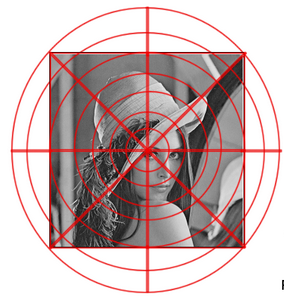
\includegraphics[width=\linewidth]{PolarImage.png}
  \caption{An image describing polar co-ordinates with image center as origin}
  \label{fig:polarCoord}
\end{figure}


\subsection{Circular Harmonics Equivariance}
We describe an image using polar co-ordinates r and $\phi$ as F(r , $\phi$). This can be understood better by looking at Figure 1. Please note that this is just to depict the polar co-ordinates of a filter. In actual setting, the filter will be applied patch-wise to the image and therefore, a single image patch will be described using these co-ordinates. \\
We will now show that there exists a filter $W_m$ such that the cross-correlation of F with $W_m$ yields a rotationally equivariant feature map. This condition is satisfied when $W_m$ is a circular harmonic of the form $W_m$ = R(r) $e^{i(m \phi + \beta)}$ for some m belonging to integers. Consider the rotation of original image by $\theta$ which leads to a new image F(r, $\phi - \theta$). The cross-correlation of the rotated image is

\vspace{-0.1cm}
\begin{center} 
[W * F(r, $\phi - \theta$)] = $\int$ W(r, $\phi$) F(r, $\phi - \theta$) dr d$\phi$ \\ \vspace{0.1cm}
$\hspace{80pt}$ = $\int$ W(r, $\phi$' + $\theta$ ) F(r, $\phi$') dr d$\phi$'
\end{center}
where $\phi$' = $\phi - \theta$. If we replace $W_m$ to be of the form R(r) $e^{i(m \phi + \beta)}$, then the integral transforms as:
\vspace{-0.1cm}
\begin{center} 
[W * F(r, $\phi - \theta$)] = $\int$ R(r) $e^{i(m (\phi' + \theta) + \beta)}$ F(r, $\phi$') dr d$\phi$' \\ \vspace{0.1cm}
$\hspace{75pt}$ = $e^{i m \theta}$ $\int$ R(r) $e^{i(m \phi' + \beta)}$ F(r, $\phi$') dr d$\phi$'
\end{center}
When rotation $\theta$ = 0, then $\phi$ = $\phi$'. Therefore, the above equation can be written as
\vspace{-0.1cm}
\begin{center} 
$\hspace{75pt}$ = $e^{i m \theta}$ $\int$ R(r) $e^{i(m \phi + \beta)}$ F(r, $\phi$) dr d$\phi$ \\ \vspace{0.1cm}
$\hspace{10pt}$ = $e^{i m \theta}$ [W * F(r, $\phi$)] 
\end{center}

\begin{figure}[t!]
  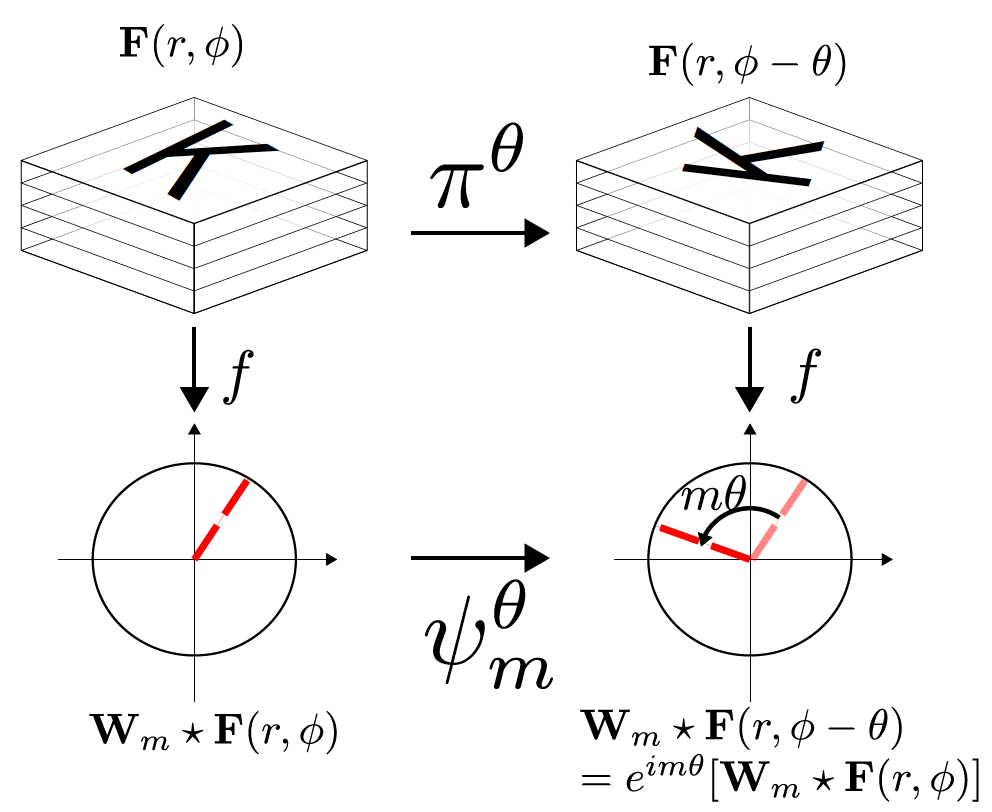
\includegraphics[width=\linewidth]{EffectOfImageRotation.png}
  \caption{Cross correlation of filter $W_m$ with non-rotated image and cross correlation of the same filter $W_m$ with an image rotated by angle $\theta$ have a defined mapping between them. We can transform the unrotated response to the rotated response via multiplication by $e^{i m \theta}$}
  \label{fig:rotatedCrossCorrelation}
\end{figure}

Hence, we observe that the cross-correlation of the rotated signal F(r, $\phi - \theta$) with harmonic filter $W_m$ = R(r) $e^{i(m \phi + \beta)}$ is equal to the response at 0 rotation [W * F(r, $\phi$)] , multiplied by a complex phase shift $e^{i m \theta}$. This is also described in figure 2. Thus, we see that cross-correlation with $W_m$ yields a rotationally equivariant feature mapping when $W_m$ is a circular harmonic. 
\subsection{Chain rule for cross-correlation of circular harmonics}
In this section, we will show that the rotation order of a feature map, obtained after subsequent cross-correlations in each layer, is equal to the sum of the rotation orders of the filters in the chain.
Let us consider cross-correlation of a $\theta$ rotated image F(r, $\phi - \theta$)  with a filter $W_m$ and then followed by another cross-correlation with $W_n$. As shown previously, we write the response of first cross-correlation as  $e^{i m \theta}$[W * F(r, $\phi$)] . Then we can write the chain rule of harmonic cross-correlation as:
\vspace{-0.1cm}
\begin{center} 
$W_n$ * [$W_m$ * F(r, $\phi - \theta$)] = $W_n$ * $e^{i m \theta}$[$W_m$ * F(r, $\phi$)] \\ \vspace{0.1cm}
$\hspace{10pt}$ = $e^{i m \theta}$($W_n$ * [$W_m$ * F(r, $\phi$)])   \\ \vspace{0.1cm}
$\hspace{10pt}$ = $e^{i m \theta} e^{i n \theta}$ [ $W_n$ * [ $W_m$ * F]]  \\ \vspace{0.1cm}
$\hspace{10pt}$ = $e^{i (m + n) \theta} $ [ $W_n$ * [ $W_m$ * F]] 
\end{center}

Therefore, we see that chained cross-correlation results in a summation of the rotation orders of the individual filters $W_m$ and $W_n$.



\subsection{Circular harmonic filter architecture}

As we described in the previous sections, a Harmonic filter is defined as $W_m$ = R(r) $e^{i(m \phi + \beta)}$, so that it can capture the rotation equivariance while classifying images. We also showed that whenever a test image is rotated, the cross-correlation of the rotated image with the learned filter, results in a product of  $e^{i m \theta}$ with [W * F(r, $\phi$)], where [W * F(r, $\phi$)] is the cross corelation with the original non-rotated test image. Hence, the classifier is able to learn that any $e^{i m \theta}$ multiple of the original cross-correlation is the same image rotated by $\theta$, and thereby classify it correctly. Therefore, this clearly defined mapping helps achieve rotation equivariance of filters, which in turn leads to global rotation invariance of the network in predicting rotated images. This is the reason, the network is able to classify rotated images with equally good accuracy.
\begin{figure}[t!]
  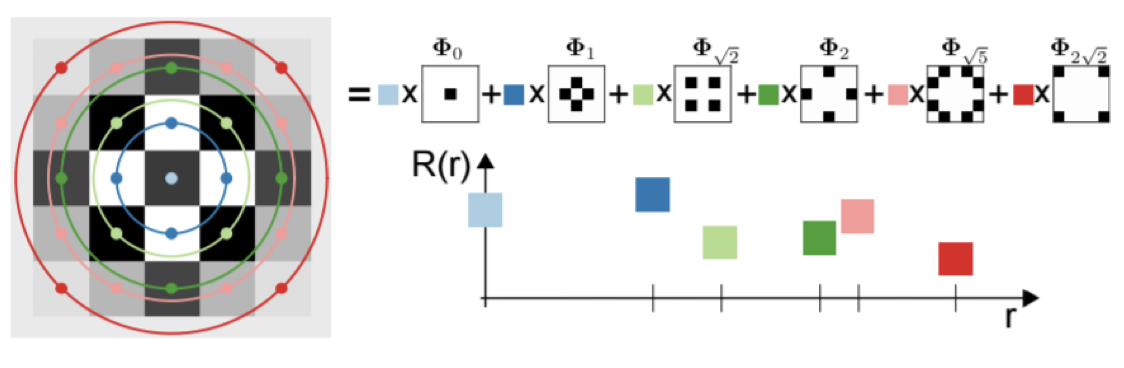
\includegraphics[width=\linewidth]{FilterArchitecture.png}
  \caption{Filter Architecture showing mapping of concentric harmonic filter profile to the cells of a square filter}
  \label{fig:FilterArch}
\end{figure}

We will now delve deeper into the architecture of a Harmonic filter.  The learnable parameters of a harmonic filter $W_m$ = R(r) $e^{i(m \phi + \beta)}$, are the radial profile R(r), which is a function of the radius r from the origin, and the per-filter phase offset $\beta$. For a n*n filter, the number of radial profile elements is equal to the number of rings of equal distance from the center of the filter. An example of this filter can be seen in Figure  \ref{fig:FilterArch}. This filter is a 5 * 5 filter with 6 rings of equal distance from the center of the filter. The smallest ring is just a single point. It is called a 5*5 filter because we are mapping the radial profile to the elements of a square filter with has length 5 and hence dimensions 5*5. Therfore, this filter has 6 radial profile terms and 1 phase offset to learn. This is in contrast to a regular convolution filter which has 25 parameters to learn ( because of 5*5 dimension of the filter). 

Now, that we have explained the architecture of the harmonic filters, there is one very important characteristic to notice. Because we are learning a complete radial profile which depends only on the radius, the filter values for a particular radial profile are same, with only difference in sign. This can be perceived as an advantage as well as a disadvantage. Advantage because this kind of constraint enables the network to learn a rotation invariant classifier. And a disadvantage because the constraint doesn't let the network learn the filter freely during training , so that it can perform the best. In the next sections, we will see how this constraining of filters serves as an advantage as well as a disadvantage when looking at different applications.

To reiterate, till now the paper gives a background of how Harmonic Networks work and how they are able to hard-bake rotation equivariance. More reference on this can be found in the paper [1]. From now on, we will discuss our main focus which describes how change in signal sparsity, signal density and noise level affects rotational equivariant features. 

\section{Parameters Affecting Rotational Equivariance}

\subsection{Noise}
Most of the image data used in real world applications are noisy in nature. One of the most important applications of image recognition and classification falls under the domain of supervision, intelligence and surveillance and despite the massive leaps in vision technology, the images captured by devices are quite noisy. While there has been good research in the fields of de-noising these images [5] , the effort and computation required outweighs the performance of such methods. 
Hence, it is quite essential to analyze the effect of noise and its variations on harmonic filters to see if it still retains its accuracy and rotation equivariance . We also framed analytical conclusions based on the theory behind harmonic filters and performed experiments to confirm our understanding.

\textbf{Types of Noise :}

An image could have multiple variations of noise incorporated into it. Some of the most common ones are :

1.	\emph{Gaussian Noise} : 

This is a form of additive noise added independently at each pixel. The added value is independent of signal intensity and is based on a gaussian distribution. One of the major reasons for this form of noise is the thermal noise (Johnson Nyquist Noise) [6]. This is one of the most common form of noise that arises due to low background illumination , increased temperature etc.

2.	\emph{Shot Noise} :

This is a noise caused due to exposure fluctuations during the time the image is captured. It is caused different counts of photons sensed at a exposure level [7]. It is dependent on the image intensity and is based on a Poisson distribution. As a result, apart from lower values of intensity its effects mimic Gaussian distribution

3.	\emph{Uniform Noise} : 

It is caused by quantizing pixels of an image to discrete levels .the distribution of such a noise is uniform.

4.	\emph{Periodic Noise} :

This noise appears as a periodic or iterating pattern over the image and is usually caused by electromagnetic interference while capturing the image.

\textbf{Analysis of effect of noise : }

For our analysis, let us assume Gaussian noise . As it is a form of additive noise [8] that is independent of intensity , the variation is induced by the general std deviation of the gaussian distribution the noise is based on . Random noise values are added to the pixels from within the gaussian distribution. 

As we start off with lower values of std deviation , the variation in the values of noise added to the pixels are not significantly large. Hence the original image can still be retrieved from the noisy image as the added noise value is nearly equal with less variation across all the pixels. 

Considering our equation in subsection 3.1, upon normalization, the harmonic filters are still able to get a multiple of the original cross correlation from the cross correlation of the noisy rotated image. The hard baked harmonic filters identify the corresponding pixel values  which although modified by a similar value throughout , are recognizable as their variation is less and hence they still retain their original pattern in the patch even after being scaled up (or down, depending on the noise added). Hence the harmonic filters perform almost as well with noise with low variance as they do without noise.

However, as the variance or std deviation of the gaussian distribution to which the noise belongs to increases , the variation of randomness in the addition of values to the pixels increases . As a result the pattern in the patch that we described earlier is lost i.e the change in pixel values are not constant and vary a lot. This makes it highly difficult for the harmonic filters to retrieve the cross correlation as a multiple of the original cross correlation. The F(r,phi) that we get here might be different from the original noiseless image .Hence it is difficult to classify the representation of the image. Although harmonic convolutions still preserve rotational equivariance, the original pattern of the image is altered and as a result the harmonic filters are not able to classify the image properly leading to lower accuracy.

This property makes the harmonic convolution exhibit similar traits as convolutional filters and hence the results reflect a similar pattern.

\textbf{Experimental Setup :}

To observe the variation in performance of the filters with noise, we chose to experiment with adding varying levels of Gaussian Noise. We used python libraries to introduce both noise and rotation in the images. To produce variation in noise levels, we kept the mean as 0 and increased the standard deviations or variance to observe the effects. 

To provide a basis of comparison for such results, we also ran a similar setup with convolutional neural networks . To further study only the effects of noise on harmonic filters and factoring out the rotational equivariance property , we also ran the experiments with non rotated noisy data on CNNs. The neural network architecture used for both the CNNs was VGG-16.
The entire experimental analysis was done on CIFAR-10 image dataset with 60k images 

\begin{figure}[t!]
  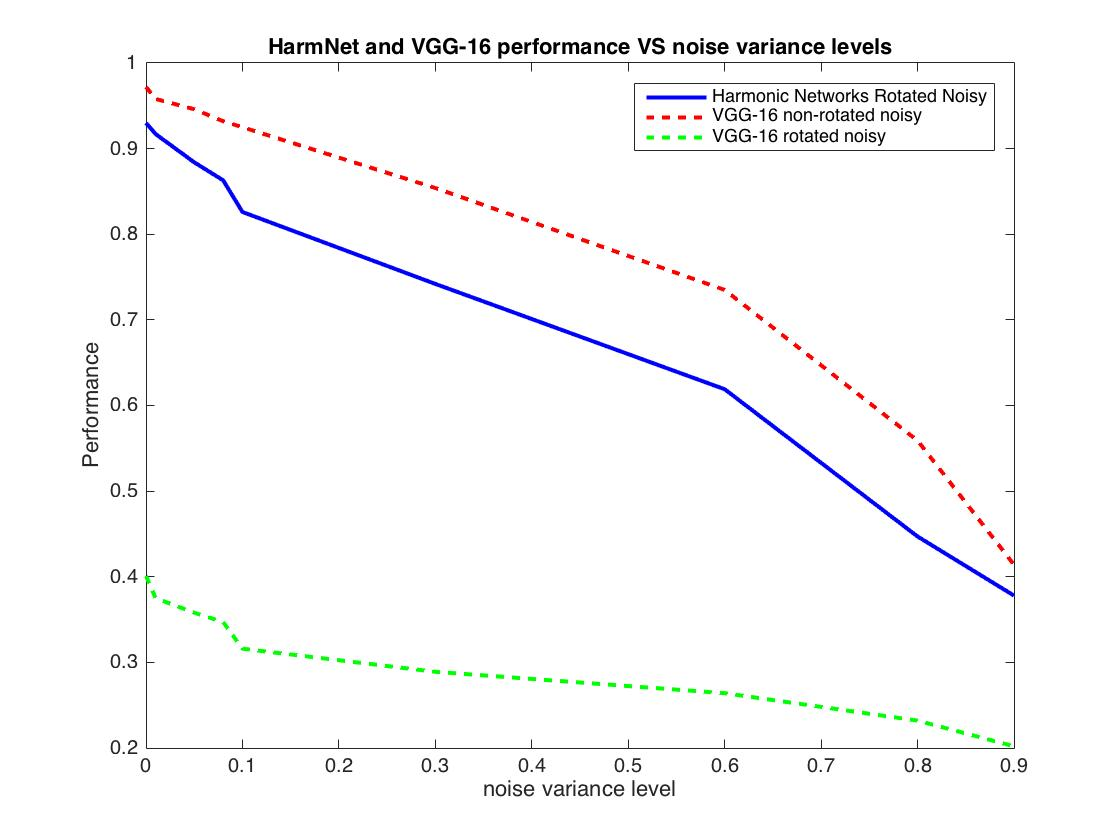
\includegraphics[width=\linewidth]{vggAndHarmVsNoise.jpg}
  \caption{Graph showing trend of accuracy with increase in noise}
  \label{fig:NoiseGraph}
\end{figure}
 
\textbf{Experimental Analysis :}

As can be observed from the graph in Fig 4 , the harmonic filters perform well in the lower values of variance in additive noise but steadily decrease as the variance increases .The same trend is observed in neural networks with non-rotated noisy images as well .An interesting point to observe is that the accuracy of harmonic filters is less by a near constant amount with respect to CNNs on non-rotated image across the entire graph. It has to be remembered that while the harmonic convolutions are on the rotated images, this CNN is on non-rotated images. The decreased performance is due to the restricted condition of the harmonic filters which learn parameters for rotation equivariance, however filters for CNN are free to learn and are unrestricted.
With same kind of data, both rotated and noisy, CNNs perform extremely poor in comparison to harmonic filters

\subsection{Sparsity}

Sparse representations of image data are widely used and recognized in the field of vision and classification experiments. Their increased popularity owing to their suitability as a regularizer for general inverse problems as well as their ease in supportability in high dimensional spaces have made them widely used in almost all image representation problems. The ease in storing and accessing sparse representations also make it highly convenient for their use. With current research showcasing increased performance in certain cases of classification with sparse representations [9] , it is highly essential that we analyze its effect on the harmonic filters to observe the change in rotation equivariance properties.

\textbf{Ways to induce sparsity in images :}

Sparse approximation problem is a highly researched topic with efficient algorithms to solve this problem in place . We list some of the most commonly used algorithms :

1.	\emph{Projected Gradient Descent} [10]: 

This is similar to normal gradient descent where the gradient shows the direction for movement. Since we are looking for a sparse solution, the putative solutions are projected onto the sparse scaffold of k vectors.

2.	\emph{ LASSO } [11] :

This regression analysis method is widely used along with its multiple variations. It solves the L1 norm version of the sparse approximation method . Fused Lasso ,Group Lasso [12] and other variations are used for generating sparsity.

3.	\emph{Proximal Methods} :

Proximal methods including proximal gradient descent is also used for induced sparsity in images .With thresholding /hard thresholding , the sparsity induced by this method forms the basis for many classification experiments.

\textbf{Analysis of Sparsity on images :}

To understand the effect of sparsity, we need to refer to the hard baked filters that are applied on patches of data. These filters as explained in the section above are concentric filters applies on pixels that in turn produce rotation equivariance. This method relies on the pattern of pixels on which the filter is applied. Now as we induce sparsity, some or most of the pixels are reduced to 0. Now, even though the pixels might not be relevant for image classification , this hinders the basic property of the pattern in the patches that the harmonic filters rely on. Hence the hard baked filters which learn in a constrained manner are not able to produce rotation equivariant features. 

We can visualize this with reference to fig 5.  where the harmonic paths are applied on a patch. Now , if we decrease the values of pixels to 0 , the purpose of the harmonic filter is defeated as with some removed pixel values , the filters do not apply on the similar kind of images as they have been trained on. As a result, in terms of cross correlation , the cross correlation value of the rotated sparse image is not a multiple of the cross correlation of the original image. Hence , the classification isn’t accurate. 

As this adversely affects the filters, the increase in sparsity should cause rapid decrease in performance of the classifier. Now, it can be observed that since these constraints are not present in the normal CNN filters , this massive decrease in performance is not observed in the case of normal convolutions. The constrained filters which produce rotation equivariance are also the cause for the decrease in accuracy of classification for harmonic convolutions .

\textbf{Experimental setup:}
 
The setup is the same as the experiments with noise. The variation in sparsity is produced by Python libraries and the percentage of sparsity is increased to observe the effect. 
The image data is CIFAR-10 with 60k images.
Similar to experiments with noise, we have kept two standard observations for comparison – CNN with non-rotated sparse images and one with rotated sparse representations.

\begin{figure}[t!]
  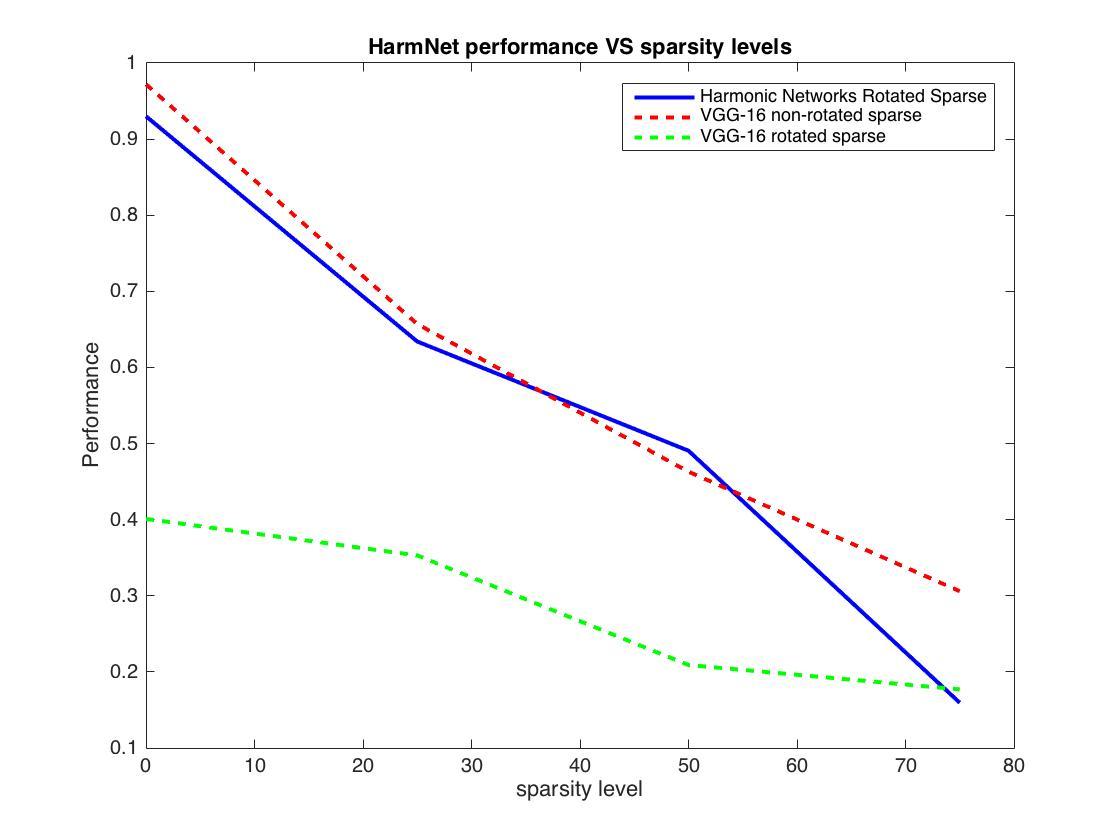
\includegraphics[width=\linewidth]{vggAndHarmVsSparse.jpg}
  \caption{Graph showing trend of sparsity with increase in noise}
  \label{fig:SparseGraph}
\end{figure}

\textbf{Experimental Results:}

As expected, there is a steep decline in the performance of the harmonic filters on increase in sparsity. With higher levels of sparsity, the filters perform poorly and lose their rotation equivariance property. Further on extremely high values of sparsity it is observed that due to the constrained filters in harmonic networks, the accuracy falls even below CNN on rotated ,sparse images. This stands as a testimony to the adverse effect of sparsity in harmonic networks.

\subsection{Quality}

Images in real world come in varying quality and cannot be expected to contain the same level of details as images used for image processing and classification in image labs in academia. For example, an image captured by a CCTV street camera is bound to be of low quality along with some inherent noise. It is, thus, important to test the efficacy of rotational equivariant features on these real world low quality images. There is yet another incentive for evaluating the performance of these features on images of varying quality. Low quality images are normally of smaller size as compared to their high-quality counterparts and consequently occupy much less disk space. Especially, if the reduction in quality is a consequence of some form of compression, the difference in size would be quite significant. If harmonic filters can be found to perform comparatively well on this image corpus of low quality rotated images, this inherent low size can be exploited to design datasets which are comparatively inexpensive to store and work with. Also the training/learning time can be considerably reduced.

\textbf{Factors affecting image quality :}

There are various ways in which the quality of an image might be affected. We focus on two important compression techniques that affect image quality :

1.	\emph{Compressed Sensing} : 

Compressed sensing or sparse sampling is a signal processing technique for efficiently acquiring and reconstructing a signal. Compressed sensing works by predicting the solutions to underdetermined linear systems of a signal. This is based on the principle that, through optimization, the sparsity of a signal can be exploited to recover it from far fewer samples than required by the Shannon-Nyquist sampling theorem. Compressed sensing builds upon the fundamental fact that we can represent many signals using only a few non-zero coefficients in a suitable basis or dictionary [13]. Nonlinear optimization can then enable recovery of such signals from very few measurements. This allows sampling/capturing images in a sparse or compressed way so as to reduce size. But the low size image sensed in this fashion is also expected to be of low quality.

2.	\emph{ JPEG Compression }:

JPEG is a lossy compression technique for digital images. The key to the JPEG baseline compression process is a mathematical transformation known as the Discrete Cosine Transform (DCT). The DCT is in a class of mathematical operations that includes Fast Fourier Transform (FFT), as well as many others. The basic purpose of these operations is to take a signal and transform it from one type of representation to another [14]. For example, an image is a two-dimensional signal that is perceived by the human visual system. The DCT can be used to convert the signal (spatial information) into numeric data ("frequency" or "spectral" information) so that the image’s information exists in a quantitative form that can be manipulated for compression.The image can then be restored to its original representational space for processing and classification. However, the compression method is lossy, meaning that some original image information is lost and cannot be restored, affecting image quality in the process.

We initially had decided to measure the effect of compressed sensing on rotational equivariant features. However, since after compressed sensing, the image representation space changes we decided, instead, to measure the effect of Discrete Cosine Transform (DCT) on rotational equivariant features using JPEG compression.


\textbf{Analysis of image Quality reduction on harmonic
filters :}

As we attempt to analyze the effect of quality on rotational equivariant harmonic filters, it is useful to remind ourselves how they fundamentally differ from the ad hoc filters in conventional convolution neural networks. As discussed in harmonic networks, the filters are hard baked to belong from the family of circular harmonics. This hard baking of filters, however, constrains the variety of filters that the network can learn. Consequently, the filter diversity of such a network is bound to be lower than the conventional convolution neural networks (CNN). This dearth in filter diversity means that the network needs to learn more filters than the convolutional CNNs, in order to perform equally accurately whilst being rotationally equivariant.

As we observed in the sections above, this constraint on filter diversity adversely affects its performance as image sparsity and noise increases. This can also be an issue when the inherent quality of the input image is quite high and hence the pixel gradient is quite steep. However, low quality images have low pixel gradient. This means that, as the quality of the image reduces, assuming that its resolution remains constant, the pixel that are adjacent to each other start taking up very similar intensity levels. This means that a network can get away with learning comparatively fewer different filters on such images. Consequently, CNNs are found to learn redundant filters on such images. This in turn should suit a harmonic network with low filter diversity. Unlike, sparsity and noise, the performance of a harmonic network should not be adversely affected as image quality decreases. Thus, we expect harmonic filters to mimic the performance of conventional CNNs whereby its accuracy plateaus as image quality keeps on reducing [2]. It is normal for CNNs to achieve this behavior as they never are constrained in the way and types of filters they are allowed to learn and hence can adjust to image quality by learning suitable filters.

This assumption, however, might not remain true as the image quality continues dropping below a certain threshold. We hypothesize, the presence of an image quality threshold below which the image is rendered indistinguishable and further reducing its quality should affect the performance of both conventional CNNs and harmonic filters much more rapidly. Below this quality threshold, the image would not have enough diverse information in its representation to be suitable to be used for the task of image classification. We now proceed to back our hypothesis with experimental evidence.

\textbf{Experimental setup:}
 
The setup environment remains the same. All experiments are conducted for 3 settings as usual, harmonic network with rotated images, CNN with rotates images and CNN on non-rotated images. The image data set used is CIFAR10, having 10 classes of images and about 60k images in total each having resolution of 32x32. The data is divided to have about 46k images in the training set, and 7k images each in the validation and test sets. The image quality is reduced by applying JPEG compression using the Python Imaging Library (PIL). PIL was also employed to randomly rotate images to feed into the rotated image configurations.

\begin{figure}[t!]
  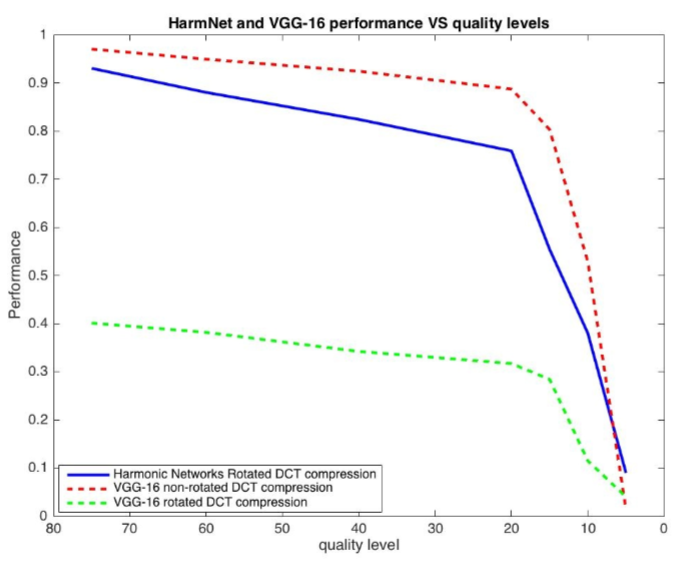
\includegraphics[width=\linewidth]{vggAndHarmVsquality.png}
  \caption{Graph showing trend of accuracy with decrease in image quality}
  \label{fig:SparseGraph}
\end{figure}

\textbf{Experimental Results:}

As hypothesized, all three configurations show similar behavior. As quality reduces from a 100 percent, the accuracy of all three configurations only plateaus, reducing by comparatively lower amounts from the initial starting point. The lower threshold for image quality is found to be in the region of 20 percent, reducing the image quality below which, induces a steep decrease in the classification accuracy of all three configurations. However, as with all previous experiments, harmonic networks outperform its CNN counterpart by a considerable margin for the rotated image configuration.


\section{Conclusion}

We’d like to conclude by saying that rotational equivariant filters hard baked from the family of circular harmonics are a significant upgrade on the unconstrained and ad hoc filters learnt by conventional CNNs. While their remains certain concerns regarding the cost of scaling networks with harmonic filter in order to increase filter diversity, their efficacy over classifying rotated images warrants further research and work with them. They perform significantly better on rotated images than their CNN counterparts in all experimental settings. Unless your domain involves dealing with highly sparse images, harmonic filters remain prime candidates to train rotational equivariant networks. Their ability to mimic CNNs immunity to quality reduction means they can also be used for classifying low quality rotated images.

\section{Future Work}
Our research clearly points out how various factors of an image like image sparsity, noise level and quality affect traditional convolutional networks in ways that do not hold true for the rotation equivariant networks. All the factors tested in this paper make sure that the images space does not change, we would like to work on how lower dimensional feature representations like compressed sensing and sketching affect harmoncic convolutions. Lower dimensional representations can also speed up the time taken to train the network and save on essential resources. Hence it would be interesting to see the tradeoffs between the use of lower dimensional representations for learning rotational equivariant features and the loss of accuracy

\section{References}
[1] Worrall, D. E., Garbin, S. J., Turmukhambetov, D., and Brostow, G. J. (2016). Harmonic Networks: Deep Translation and Rotation Equivariance. arXiv preprint arXiv:1612.04642.

[2] Dodge, S., and Karam, L. (2016, June). Understanding how image quality affects deep neural networks. In Quality of Multimedia Experience (QoMEX), 2016 Eighth International Conference on (pp. 1-6). IEEE.

[3] Rigamonti, R., Brown, M. A., and Lepetit, V. (2011, June). Are sparse representations really relevant for image classification?. In Computer Vision and Pattern Recognition (CVPR), 2011 IEEE Conference on (pp. 1545-1552). IEEE.

[4] Zabala, A., Pons, X., Díaz-Delgado, R., García, F., Aulí-Llinàs, F., and Serra-Sagristà, J. (2006, July). Effects of JPEG and JPEG2000 lossy compression on remote sensing image classification for mapping crops and forest areas. In Geoscience and Remote Sensing Symposium, 2006. IGARSS 2006. IEEE International Conference on (pp. 790-793). IEEE.

[5] Russo, F. (2003). A method for estimation and filtering of Gaussian noise in images. IEEE Transactions on Instrumentation and Measurement, 52(4), 1148-1154.

[6] Landauer, R. (1989). Johnson-Nyquist noise derived from quantum mechanical transmission. Physica D: Nonlinear Phenomena, 38(1-3), 226-229.

[7] Brida, G., Genovese, M., and Berchera, I. R. (2010). Experimental realization of sub-shot-noise quantum imaging. Nature Photonics, 4(4), 227-230.

[8] Olsen, S. I. (1993). Estimation of noise in images: An evaluation. CVGIP: Graphical Models and Image Processing, 55(4), 319-323.

[9] Yang, J., Yu, K., Gong, Y., and Huang, T. (2009, June). Linear spatial pyramid matching using sparse coding for image classification. In Computer Vision and Pattern Recognition, 2009. CVPR 2009. IEEE Conference on (pp. 1794-1801). IEEE.

[10] Chen, X., Lin, Q., Kim, S., Carbonell, J. G., and Xing, E. P. (2012). Smoothing proximal gradient method for general structured sparse regression. The Annals of Applied Statistics, 719-752.

[11] Tibshirani, Robert, et al. "Sparsity and smoothness via the fused lasso." Journal of the Royal Statistical Society: Series B (Statistical Methodology) 67.1 (2005): 91-108.

[12] Friedman, J., Hastie, T., and Tibshirani, R. (2010). A note on the group lasso and a sparse group lasso. arXiv preprint arXiv:1001.0736.

[13] Davenport, M. A., Duarte, M. F., Eldar, Y. C., and Kutyniok, G. (2011). Introduction to compressed sensing. Preprint, 93(1), 2.
 
[14] Chen, W., Wilson, J., Tyree, S., Weinberger, K. Q., and Chen, Y. (2016, August). Compressing convolutional neural networks in the frequency domain. In Proceedings of the 22Nd ACM SIGKDD International Conference on Knowledge Discovery and Data Mining, ser. KDD’16 (pp. 1475-1484).


% In the unusual situation where you want a paper to appear in the
% references without citing it in the main text, use \nocite
\nocite{langley00}

\bibliography{example_paper}
\bibliographystyle{icml2017}

\end{document} 


% This document was modified from the file originally made available by
% Pat Langley and Andrea Danyluk for ICML-2K. This version was
% created by Lise Getoor and Tobias Scheffer, it was slightly modified  
% from the 2010 version by Thorsten Joachims & Johannes Fuernkranz, 
% slightly modified from the 2009 version by Kiri Wagstaff and 
% Sam Roweis's 2008 version, which is slightly modified from 
% Prasad Tadepalli's 2007 version which is a lightly 
% changed version of the previous year's version by Andrew Moore, 
% which was in turn edited from those of Kristian Kersting and 
% Codrina Lauth. Alex Smola contributed to the algorithmic style files.  
